\section{Bases de datos orientadas a Grafos (BDOG o Graph Databases)}

\begin{frame}
\frametitle{Introducción}
\begin{itemize}

\item	Algunas aplicaciones requieren guardar grafos gigantescos de
	forma segura y manipularlos eficientemente.
	\pause

\item	Como siempre, se puede usar un motor relacional y manejar
	la lógica a nivel de aplicación. Se podrían incluso usar índices
	para acelerar los joins (que representarían la búsqueda de vecinos)
	a costo de updates mas lentos y espacio en disco.
	\pause

\item	Una BDOG se define como una base de datos que provee ``adjacencia
	sin uso de índices'', o sea, que maneja los grafos de una manera
	\textit{natural} y \textit{eficiente}.
	\pause

\item	De esta manera, se prestan a modelar datos heterogéneos y
	conectados.
\end{itemize}
\end{frame}

\begin{frame}
\frametitle{Un poco de autobombo}
\begin{itemize}
\item	We live in a connected world. There are no isolated pieces of
	information, but rich, connected domains all around us. Only a database
	that embraces relationships as a core aspect of its data model is able
	to store, process, and query connections efficiently. \textbf{While other
	databases compute relationships expensively at query time, a graph
	database stores connections as first class citizens, readily available
	for any “join-like” navigation operation.} Accessing those already
	persistent connections is an efficient, constant-time operation and
	allows you to quickly traverse millions of connections per second per
	core.
\end{itemize}
\end{frame}

\begin{frame}
\center
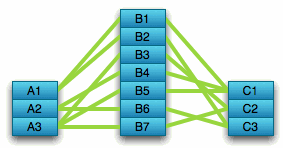
\includegraphics[width=0.9\linewidth,height=0.9\textheight,keepaspectratio]{bdog-1}
\end{frame}
\begin{frame}
\center
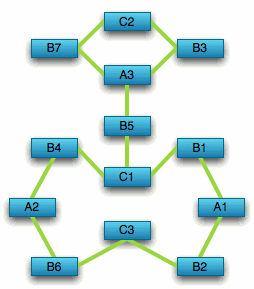
\includegraphics[width=0.9\linewidth,height=0.9\textheight,keepaspectratio]{bdog-2}
\end{frame}

\begin{frame}
\frametitle{Implementando un KV store}
 \center
 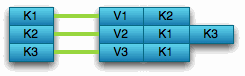
\includegraphics[width=0.9\linewidth,height=0.9\textheight,keepaspectratio]{bdog-3}
\end{frame}

\begin{frame}
\frametitle{Implementando un KV store}
 \center
 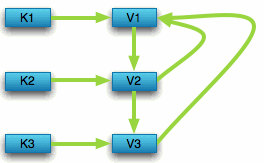
\includegraphics[width=0.9\linewidth,height=0.9\textheight,keepaspectratio]{bdog-4}
\end{frame}

\begin{frame}
\frametitle{Características}
\begin{itemize}
\item	En una BDOG, nunca puede haber una relación sin ambos nodos
	que conecta (\textit{No broken links}).
	\pause

\item	Pueden tener consistencia ACID (Neo4j la tiene).
\end{itemize}
\end{frame}

\section{Neo4j}

\begin{frame}
\frametitle{Neo4j}
\begin{itemize}
\item	Neo4j es un GDBMS open-source, con una versión gratuita y una
	paga, que implementa este modelo.
	\pause

\item	Usada por muchísimas empresas y organizaciones (eBay, Walmart,
	Cisco, y más).
\end{itemize}
\end{frame}
